% !TeX spellcheck = en_GB
% !TeX encoding = UTF-8 

\documentclass[14pt,a4paper]{extarticle}

\usepackage[english]{babel}
\usepackage[utf8]{inputenc}
\usepackage{setspace} 
\usepackage[a4paper,
	left=30mm,
	right=10mm,
	top=20mm,
	bottom=20mm]{geometry}
\usepackage{amsmath,amssymb,amsthm}
\usepackage{cite}
\usepackage{graphicx} 
\usepackage{subfigure,subcaption}
\usepackage{kprjHSE} 
\usepackage{tikz}
\usepackage{xcolor,tabularray}
\usepackage{wrapfig}

\usetikzlibrary{positioning}

\renewcommand{\labelenumii}{\arabic{enumi}.\arabic{enumii}}

\lstset{
	frame=single,
	basicstyle=\ttfamily,
	breaklines=true,
	tabsize=4
}

\LabWork
\LabWorkNo{3}

\setcounter{MaxMatrixCols}{20}

\FirstAuthor{M.D.~Kirdin}
\FirstConsultant{A.~Tomat}
\SecondConsultant{M.~Zueva}
\discipline{Ordered Sets for Data Analysis}
\faculty{Faculty of Computer Science}
\chair{School of Data Analysis and Artificial Intelligence}
\chief{S.O.~Kuznetsov}
\workyear{2024}

\onehalfspacing

\begin{document}
	\maketitle
	
	\subsection*{Question 1}
	\noindent\textbf{Task.} For the context given in the following table:
	\begin{enumerate}
		\item find all formal concepts using the CbO algorithm (show the tree);
		\item draw the concept lattice.
	\end{enumerate}
	
	\begin{center}
		\begin{tblr}{width=.45\linewidth,
				colspec={|X[c]|X[c]|X[c]|X[c]|X[c]|X[c]|}
				}
			\hline
			  & a & b & c & d & e\\
			\hline
			1 &  & 1 & 1 &   &  \\
			\hline
			2 & 1 & 1 & 1 &   & 1\\
			\hline
			3 & 1 & 1 &   & 1 &  \\
			\hline
			4 & 1 &   &   & 1 & 1\\
			\hline
		\end{tblr}
	\end{center}
	 
	\noindent\textbf{Solution.} Let's draw the concept lattice.
	
	\begin{figure}[h]
		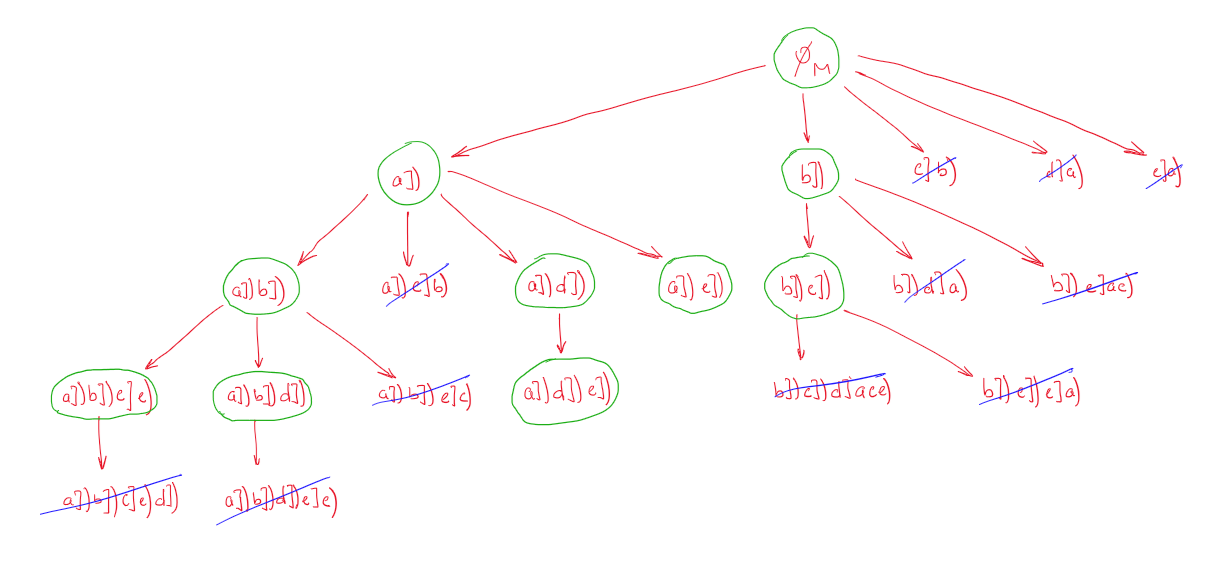
\includegraphics[width=\textwidth]{media/task1.png}
		\centering
		\caption{Concept lattice produced by CbO algorithm}
		\label{fig:CbO}
	\end{figure}
	
	On \figref{fig:CbO} green circles indicate formal concepts and blue strikethroughs indicate non-canonical intent generations. From it we can infer that there are following formal concepts: $(G,\, \emptyset_M)$, $(\{2,\,3,\,4\},\, \{a\})$, $(2,\, \{a,\, b,\, c,\, e\})$, $(3,\, \{a,\, b,\, d\})$, $(\{3,\, 4\},\, \{a,\, d\})$, $(4, \{a,\, d,\, e\})$, $(\{2,\, 4\},\, \{a,\, e\})$, $(\{1,\, 2,\, 3\},\, b)$, $(\{1,\, 2\}, \{b,\, c\})$.
	
	\newpage
	\subsection*{Question 2}
	
	\noindent\textbf{Task.} For the following many-valued context given in the following table:
	
	\begin{enumerate}
		\item Binarize the data given in the table. Use nominal scales for the features (Brand, Color). For the feature (RAM), use the ordinal scale ($\geq8$, $\geq16$, $\geq32$) given in the table on the right. For the feature (is\textunderscore{touch}), use the dichotomic scale (is\textunderscore{touch}, not is\textunderscore{touch}).
		\item Find the minimal positive and minimal negative hypotheses of the binarized context. (Show the concept lattices of both the positive and negative contexts).
		\item Classify the objects <Razer, Black, 32, Yes>, <Toshiba, Red, 18, Yes>, <Mac, Pink, 8, No> using the found hypotheses.
	\end{enumerate}
	
	\begin{center}
		\begin{tblr}{width=0.65\linewidth,
				colspec={|X[c]|X[c]|X[c]|X[c]|X[c]|}
			}
			\hline
			Brand & Colour & RAM & is\textunderscore{}touch & class\\
			\hline
			Lenovo & Black & 16 & No & +\\
			\hline
			HP & Black & 16 & Yes & +\\
			\hline
			Lenovo & Black & 16 & Yes & +\\
			\hline
			Razer & Silver & 32 & No & +\\
			\hline
			Razer & Gold & 32 & No & +\\
			\hline[1pt]
			Toshiba & Pink & 4 & Yes & -\\
			\hline
			Toshiba & White & 16 & Yes & -\\
			\hline
			HP & Silver & 8 & No & -\\
			\hline
			Mac & Gold & 16 & No & -\\
			\hline
		\end{tblr}
	\end{center}
	
	\begin{center}
		\begin{tblr}{width=.4\linewidth,
				colspec={|X[c]|X[c]|X[c]|X[c]|}
			}
			\hline
			 & $\geq8$ & $\geq16$ & $\geq32$\\
			\hline
			4 &  &  & \\
			\hline
			8 & 1 &  & \\
			\hline
			16 & 1 & 1 & \\
			\hline
			32 & 1 & 1 & 1\\
			\hline
		\end{tblr}
	\end{center}
	\newpage
	
	\noindent\textbf{Solution.} Binarized data can be seen in table below:
	 
	\rotatebox{90}{\fontsize{11pt}{12pt}\selectfont
		\begin{tblr}{width=.96\textheight,
				colspec={|X[c]|X[c]|X[c]|X[c]|X[c]|X[c]|X[c]|X[c]|X[c]|X[c]|X[c]|X[c]|X[c]|X[c]|X[c]|X[c]|X[c]|}
			}
			\hline
			   & len & hp & raz & tsb & mac & blk & sil & gol & pnk & wht & $\geq8$ & $\geq16$ & $\geq32$ & tch\textunderscore{y} & tch\textunderscore{n} & class\\
			\hline
			 1 & + & - & - & - & - & + & - & - & - & - & + & + & - & - & + & + \\
			 \hline
			 2 & - & + & - & - & - & + & - & - & - & - & + & + & - & + & - & + \\
			 \hline
			 3 & + & - & - & - & - & + & - & - & - & - & + & + & - & + & - & + \\
			 \hline
			 4 & - & - & + & - & - & - & - & - & - & - & + & + & + & - & + & + \\
			 \hline
			 5 & - & - & + & - & - & - & - & + & - & - & + & + & + & - & + & + \\
			 \hline[1.5pt]
			 6 & - & - & - & + & - & - & - & - & + & - & - & - & - & + & - & - \\
			 \hline
			 7 & - & - & - & + & - & - & - & - & - & + & + & + & - & + & - & - \\
			 \hline
			 8 & - & + & - & - & - & - & + & - & - & - & + & - & - & - & + & - \\
			 \hline
			 9 & - & - & - & - & + & - & - & + & - & - & + & + & - & - & + & - \\
			 \hline[1pt]
			10 & - & - & + & - & - & + & - & - & - & - & + & + & + & + & - & $\tau$ \\
			 \hline
			11 & - & - & - & + & - & - & - & - & - & - & + & + & - & + & - & $\tau$ \\
			 \hline
			12 & - & - & - & - & + & - & - & - & - & - & + & - & - & - & + & $\tau$ \\
			 \hline
		\end{tblr}
	}
	\newpage
	Using this data we can construct positive and negative concept lattices.
	
	\begin{figure}[h]
		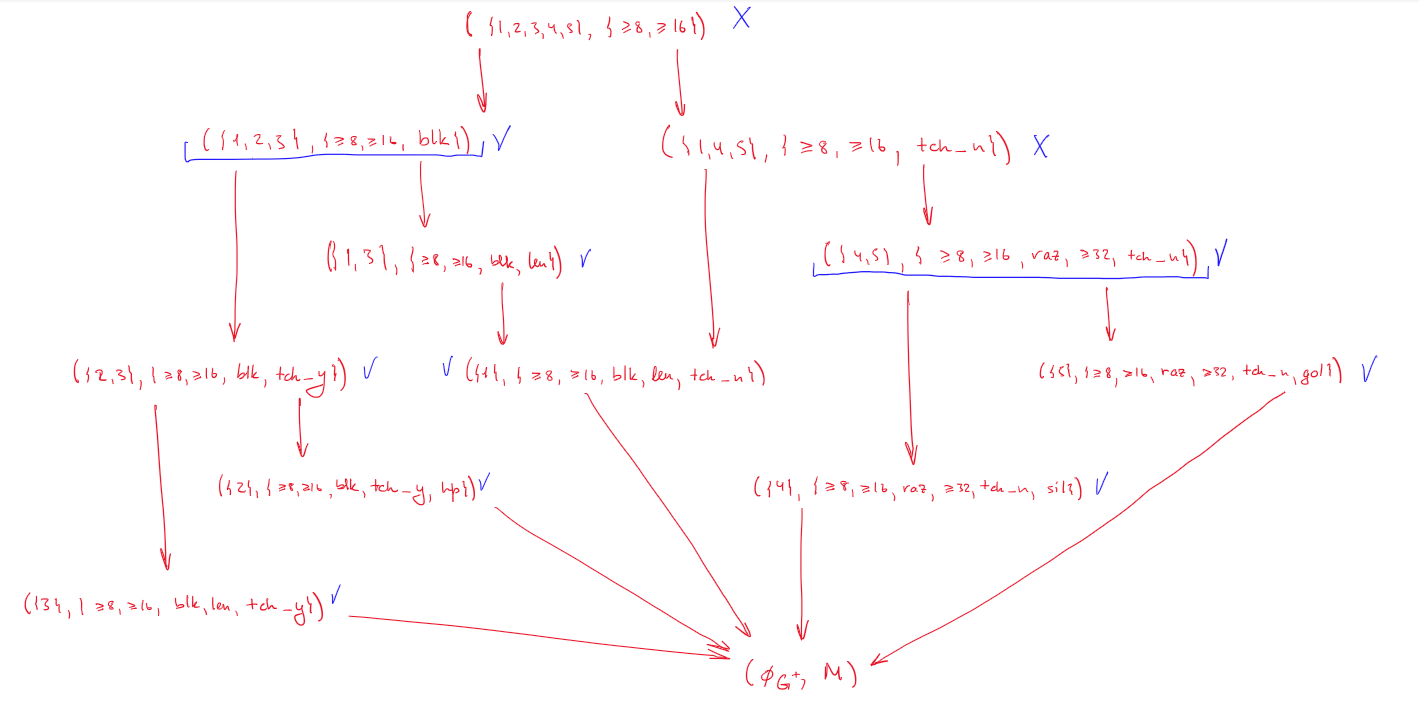
\includegraphics[scale=.4]{media/task2_1.png}
		\centering
		\caption{Positive concept lattice}
		\label{fig:pos_lat}
	\end{figure}
	
	\begin{figure}[h]
		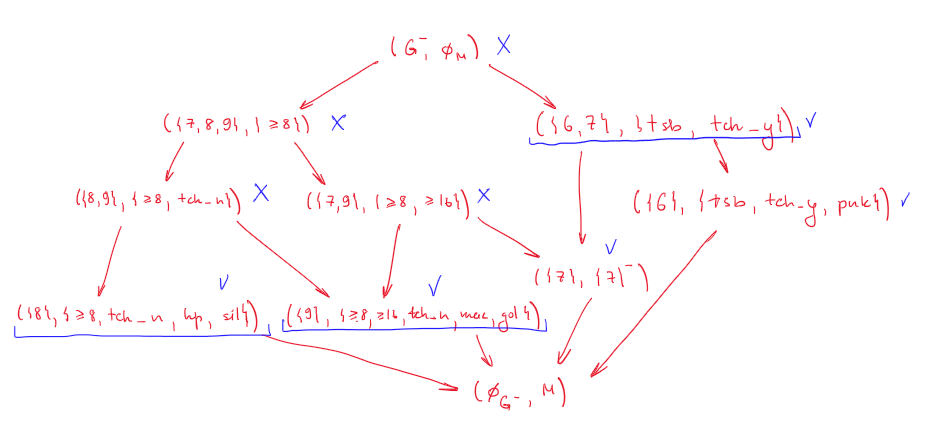
\includegraphics[scale=.6]{media/task2_2.png}
		\centering
		\caption{Negative concept lattice}
		\label{fig:neg_lat}
	\end{figure}
	
	According to \figref{fig:pos_lat}, \{$\geq8$, $\geq16$, blk\} and \{$\geq8$, $\geq16$, $\geq32$, raz, tch\textunderscore{n}\} are minimal positive hypotheses. \{$\geq8$, $\geq16$\} is not a positive hypothesis since it is part of a negative hypothesis. Those, according to \figref{fig:neg_lat} are: \{tsb, tch\textunderscore{y}\}, \{$\geq8$, tch\textunderscore{}n, hp, sil\}, \{$\geq8$, $\geq16$, tch\textunderscore{}n, mac, gol\}. Therefore, since:
	\begin{itemize}
		\item $\{10\}^{\tau}$ contains \{$\geq8, \geq16$, blk\} and no negative hypotheses, 10 is a positive observation;
		\item $\{11\}^{\tau}$ contains \{tsb, tch\textunderscore{y}\} and no positive hypotheses, 11 is a negative observation;
		\item $\{12\}^{\tau}$ does not contain any positive or negative observations, 12 should be labelled as undetermined.
	\end{itemize}
\end{document}